\section{Results}
\label{s:results}
\cbstart
This Chapter is divided into multiple parts and starts off with the conceptual results first. Afterwards, all technical details including the requirements of the practical application are discussed. The details consist of two Sections dealing with automatic data acquisition and preprocessing. With the successful acquisition and preparation, the web application can be discussed. The most important tools are listed and their main purpose for the implementation is shown. The Chapter is concluded with the results of the conducted user study showing the effectiveness of the animated transitions.
\cbend

\subsection{Requirements}
The practical application needs to meet some basic conditions, which are described below:

\begin{description}
\item[Scaling:] unit-based visualisations allow for showing a lot of items simultaneously and combined with animation, some patterns in data can be revealed. However, using a low amount of units will not result in showing patterns animations. Therefore, using a mid-sized dataset is a key part of the practical implementation. Defining a mid-sized dataset is nebulous and for this thesis, it is defined as a dataset consisting of 5000 to 15000 rows. This amount should be enough for an experiment to investigate the question of how an aggregation can be realized.

\item[Modularity:] the practical implementation should have a modular structure in order to keep it extendable. It should be possible to add further visualisations and transitions for more investigation later on.

\item[Client-side application:] in order to save costs and abstractions, a client-side approach is required. This allows to put the focus on the implementation of different thematic maps and an animated transition between them without worrying about latency of server response.

\end{description}

\subsection{Data Acquisition}
\label{s:data-acquisition}
Tableau uses a very interesting sample dataset to show basic features. It is called "Superstore-Sale" and contains approximately 10000 rows. Superstore-Sale features a lot of different attributes for each item. It comes close to the example of e-commerce mentioned in chapter \ref{s:geovis-practical} on page \pageref{s:geovis-practical}. The dataset mainly consists of information about office products, which have been bought in the period of time from 2011 to 2014. Furthermore each order in the dataset includes some parts of the delivery address. This information about country, city, state and postal code allows to use the dataset with a map because it features some kind of geographical information. However, before being able to use the dataset on a map, it must be expanded by longitude and latitude first. This part is explained in detail in section \ref{s:data-preprocessing} on page \pageref{s:data-preprocessing}.

Having a dataset with interesting information leads to the second part of this section. A thematic map does not only consist of its symbols or coloured areas, it also needs to show the geographical conditions in form of a map. "Superstore-Sale" only includes items from the United States, thus a map of this location is needed. The U.S. Census Bureau publishes cartographic boundaries as shapefiles for thematic mapping. They provide multiple resolutions for different use cases. For the chosen dataset, the lowest resolution will show enough features in the map. Being able to see forests, streets, and so forth, in the map is not needed to show an overview of a commercial dataset. An advantage using a low resolution dataset is the file size. This must be considered, because we will put all information to the client, thus delivering 1 \ac{mb} or 100\ac{mb} of information is significant in terms of loading time of the web application.
Furthermore, the topicality of the cartographic boundaries needs to be considered. Usually county boundaries do not change frequently, so it is acceptable to use the decennial census rather than the most recent release. Listing \ref{lst:data-acqu-zip} on page \pageref{lst:data-acqu-zip} shows an automated way of downloading the decennial version of the lowest resolution cartographic boundaries. It is accomplished with GNU-Make\footnote{See \href{https://www.gnu.org/software/make/}{GNU Make} for more information.}. The target name without the directory, \textit{gz_2010_us_050_00_20m}, implicitly has some information:

\begin{lstlisting}[style={make-pretty}, caption={Make task for downloading cartographic boundaries}, label={lst:data-acqu-zip}]
build/gz_2010_us_050_00_20m.zip:
    mkdir -p \$(dir \$\@)
    curl -o \$\@ http://www2.census.gov/geo/tiger/GENZ2010/\$(notdir \$\@)
\end{lstlisting}

\begin{itemize}
\item \textit{2010} is the release year of the file
\item \textit{us} refers to boundaries of the united states
\item \textit{20m} denotes the resolution (1:20.000.000)
\end{itemize}

The mentioned make task will download the zip-file from the census bureau and save it in the build directory.



\subsection{Data Preprocessing}
\label{s:data-preprocessing}
As the section before already showed, two different files are now accessible. However, in order to actually use these files, some preprocessing is needed. This chapter is divided into three parts. The first one will discuss the preparation of the Superstore-Sale dataset, the second one will explain how to get boundaries out of the downloaded zip-file, and the third one will demonstrate how these two files can be merged.

\subsubsection{Preprocessing Superstore-Sale}
First of all, some numbers in this dataset are shown in a different format. Converting all numbers to the same format is essential.
Secondly, as already mentioned, the dataset only features attributes like country, city, state and postal code. In order to show the items on the map, it is necessary to expand each item with longitude and latitude. Listing \ref{lst:data-prep-latlong} on page \pageref{lst:data-prep-latlong} shows how the expansion can be accomplished when using NodeJs\footnote{See \href{https://nodejs.org/en/}{NodeJs} for more information.}. The listing uses Nominatim\footnote{See \href{https://nominatim.openstreetmap.org/}{Nominatim} for more information.} to decode geographical location strings to longitude and latitude. Furthermore listing \ref{lst:data-prep-latlong} shows, that each item is extended two more attributes: \textit{CountyId} and \textit{StateId}. These attributes denote the geographical id to the corresponding county and state name. As a starting point, a file containing all zip-codes with their corresponding ids was needed. Jgoodall provides such a file in his us-map repository\footnote{See \href{https://github.com/jgoodall/us-maps/}{this repository} for more information.}. Reading this file results in a lookup dictionary, where it is possible to search each postal code for its corresponding ids. However, Superstore-Sale does not provide a leading zero if a postal code is less than five characters, leading to a special case, which has to be considered.

%TC:ignore
\begin{lstlisting}[language=JavaScript, caption={Preprocessing Superstore-Sale with latitude and longitude}, label={lst:data-prep-latlong}]
let zipCodes = require("./zip-codes.json");
// Add latitude and longitude if there is a geo information
if (item.hasOwnProperty("Country") && item.hasOwnProperty("City") && item.hasOwnProperty("State")) {
    let url = `http://nominatim.openstreetmap.org/search?email=${config.email}&format=json&`;
    url += `country=${item.Country}&`;
    url += `state=${item.State}&`;
    url += `city=${item.City}`;

    const response = request("GET", url, {
        "headers": {
            "user-agent": "University of Applied Sciences Salzburg - Masterthesis Particles - MMT-M2014"
        }
    });
    const data = JSON.parse(response.getBody());
    item.Latitude = data[0].lat;
    item.Longitude = data[0].lon;
}

if (item.hasOwnProperty("Postal Code")) {
    let currentZip = item["Postal Code"];
    if(zipCodes.hasOwnProperty(currentZip)){
        let codes = zipCodes[currentZip];
        item.CountyId = codes.countyId[0];
        item.StateId = codes.stateId;
    } else {
        // superstore has no leading 0 of postal codes if code length < 5;
        currentZip = "0".concat(currentZip)
        if(zipCodes.hasOwnProperty(currentZip)){
            let codes = zipCodes[currentZip];
            item.CountyId = codes.countyId[0];
            item.StateId = codes.stateId;
        }
    }
}
\end{lstlisting}
%TC:endignore

\subsubsection{Preprocessing Cartographic Boundaries}
Section \ref{s:data-acquisition} on page \pageref{s:data-acquisition} already mentions how to automatically download and save the zip file containing cartographic boundaries of the United States. However, the zip-file by itself is not useful. The contents of the zip-file need to be converted first in order to actually being able to use the data. Listing \ref{lst:data-acqu-unzip} on page \pageref{lst:data-acqu-unzip} displays the make task for unzipping files. This task unzips \textit{gz\_2010\_us\_050\_00\_20m.zip} resulting in \textit{gz\_2010\_us\_050\_00\_20m.shp}. A shapefile is a common standard\footnote{See \href{https://doc.arcgis.com/en/arcgis-online/reference/shapefiles.htm}{the definition of a shapefile} for more information} for representing geospatial vector data.

%TC:ignore
\begin{lstlisting}[style={makefile}, caption={Make task for unzipping files}, label={lst:data-acqu-unzip}]
/*build/gz_2010_us_050_00_20m.shp*/: build/gz_2010_us_050_00_20m.zip
    unzip -od $(dir $@) $<
    touch $@
\end{lstlisting}
%TC:endignore

However, shapefiles cannot be used directly in today's browsers. Converting it to GeoJSON\footnote{See \href{http://geojson.org/}{GeoJSON} for more information.} first yields the result of having a usable file in the browser. GeoJSON is a format for encoding a variety of geographic data structures in a JSON structure. There are a variety of tools available converting shapefiles to GeoJSON. In order still automatize it, a command-line tool is needed, and therefore TopoJSON\footnote{See \href{https://github.com/mbostock/topojson}{TopoJSON} for more information.} was used. TopoJSON is a simple extension to GeoJson that encodes topology. Listing \ref{lst:data-acqu-topo1} on page \pageref{lst:data-acqu-topo1} shows the usage of this command line tool. The option \textit{-o} simply denotes the input file, \textit{--} tells TopoJSON that all options are passed in and \textit{counties} is the JSON-key all information is put in.

%TC:ignore
\begin{lstlisting}[style={makefile}, caption={Make task for converting shapefiles to geojson}, label={lst:data-acqu-topo1}]
/*data/counties.json*/: build/gz_2010_us_050_00_20m.shp
    node_modules/.bin/topojson \
        -o $@ \
        -- counties=$<
\end{lstlisting}
%TC:endignore

With this task, a file containing all cartographic boundaries for all counties exists. If this level of detail is too high, listing \ref{lst:data-acqu-topo2} and \ref{lst:data-acqu-topo3} on page \pageref{lst:data-acqu-topo2} and \pageref{lst:data-acqu-topo3} show how to create a file containing all state boundaries or only the main country boundaries. The \textit{--key='d.id.substring(d.id.search("S")+1, d.id.search("S")+3)'} is the aggregation base. Each item has an id which simply is the geo-id of the county. This geo-id is a combination of state-id and county-id and therefore using a substring of this id can be used to aggregate counties in the same state resulting in state boundaries.

%TC:ignore
\begin{lstlisting}[style={makefile}, caption={Make task for aggregating counties to states by state-id}, label={lst:data-acqu-topo2}]
/*data/states.json*/: data/counties.json
    ./../node_modules/.bin/topojson-merge \
        -o $@ \
        --in-object=counties \
        --out-object=states \
        --key='d.id.substring(d.id.search("S")+1, d.id.search("S")+3)' \
        -- $<
\end{lstlisting}

%TC:ignore
\begin{lstlisting}[style={makefile}, caption={Make task for converting state boundaries to a county boundary}, label={lst:data-acqu-topo3}]
/*data/us.json*/: data/states.json
    ./../node_modules/.bin/topojson-merge \
        -o $@ \
        --in-object=states \
        --out-object=country \
        -- $<
\end{lstlisting}
%TC:endignore

\subsubsection{Merging Superstore-Sale with Cartographic Boundaries}
This section mainly discusses pre-processing steps of one of the two methods mentioned to implement an aggregated thematic map (see chapter \ref{s:web-application} on page \pageref{s:web-application} for more information). The objective of merging Superstore-Sale with the already preprocessed boundary-files is to have one file including all aggregated values of orders per county or state. Such a file can be used to show all orders for each county or state without the need of dynamically calculating it.
In order to aggregate the orders on a county level of detail, listing \ref{lst:data-acqu-topo1} on page \pageref{lst:data-acqu-topo1} needs some adaptations with a new starting file. Using the already preprocessed Superstore-Sale dataset, it is possible to create a new file with the aggregated information. Listing \ref{lst:data-prep-amount} on page \pageref{lst:data-prep-amount} iterates the given dataset, creates a county-based dictionary counting all objects having the same county and writes the information back to a file.

%TC:ignore
\begin{lstlisting}[language=JavaScript, caption={Creating the file containing aggregation information}, label={lst:data-prep-amount}]
csv.fromPath("./path-to-preprocessed-superstore-sale.csv", {
    headers: true,
    delimiter: ";"
})
.on("data", function(item){

    let countyKey = `${item.StateId}${item.CountyId}`;
    countyDict[countyKey] = ++countyDict[countyKey] || 1;

})
.on("end", function(){

    let result = [];

    result.push([
        "GEO_ID",
        "ID",
        "AMOUNT"
    ]);

    for (let [key,value] of objectEntries(countyDict)) {
        result.push([
            `0500000US${key}`,
            `${key}`,
            `${value}`
        ]);
    }

    let ws = fs.createWriteStream(
        "./data/superstore-aggregated.csv",
        {encoding: "utf8"}
    );
    // comma seperation needed because of topojson
    csv.write(result, {headers: true, delimiter: ","}).pipe(ws);
});
\end{lstlisting}
%TC:endignore

This listing yields a file which can be used in combination with the already created topojson file. Listing \ref{lst:data-acqu-topo4} on page \pageref{lst:data-acqu-topo4} is an updated version of listing \ref{lst:data-acqu-topo1} on page \pageref{lst:data-acqu-topo1}. It extends the already mentioned task by combining the newly created aggregation file. The option \textit{--id-property} simply denotes the identification key for each item for both files. All \textit{--external-properties} needs a file as input parameter to look up \textit{--properties} which cannot be found in the original input file from the task. Thus, all \textit{--properties} listed in the task are available as a key-value pair later on.

%TC:ignore
\begin{lstlisting}[style={makefile}, caption={Make task for merging a file with topojson}, label={lst:data-acqu-topo4}]
/*data/counties.json*/: build/gz_2010_us_050_00_20m.shp
    ./../node_modules/.bin/topojson \
        -o $@ \
        --id-property 'GEO_ID' \
        --external-properties ./data/superstore-aggregated.csv \
        --properties 'geoId=GEO_ID' \
        --properties 'stateId=STATE' \
        --properties 'countyId=COUNTY' \
        --properties 'county=NAME' \
        --properties 'orders=AMOUNT' \
        -- counties=$<
\end{lstlisting}
%TC:endignore


\subsection{Used technologies}
The web-application is written in JavaScript ES6\footnote{See \href{http://www.ecma-international.org/ecma-262/6.0/}{http://www.ecma-international.org/ecma-262/6.0/} for more information.}. The development is done under Linux and the application is tested on Linux and Windows.

\subsubsection{D3}
D3.js\footnote{See \href{https://d3js.org/}{https://d3js.org/} for more information.} is a library based on JavaScript. It allows to bind arbitrary data to a \ac{DOM}, and apply transformations to the document afterwards. \ac{D3} makes use of \ac{HTML}, \ac{SVG} and \ac{CSS}. Using these web standards offers full capabilities of modern browsers. It includes powerful visualisation components and data-driven approach to \ac{DOM} manipulation. \ac{D3} is supposed to be really fast, supporting large datasets and dynamic behaviours for interaction and animation. The component-based architecture of \ac{D3} allows for code reuse. Furthermore, it allows for developing plugins rather easily.

The practical application uses \ac{D3} for two differnt things:
\begin{enumerate}
\item The base map is drawn using \ac{D3} because it features a lot of different map projections, allows to use the client-side library of TopoJSON, and overall has a lot of useful interactions implemented already.
\item All thematic maps based on aggregation are realised with \ac{D3} because of its use of \ac{SVG} and the interaction.
\end{enumerate}

\subsubsection{PixiJS}
\ac{Pixi} is a fast and lightweight 2D library\footnote{See \href{http://www.pixijs.com/}{http://www.pixijs.com/} for more information.} built upon Canvas technology. Its renderer allows to enjoy e.g. hardware acceleration without the prior knowledge of \ac{WebGL}. Thus, \ac{Pixi} simplifies the creation of rich, interactive, cross platform applications without the need of knowledge of browser and device compatibility. Another characteristic of \ac{Pixi} is the seamless fallback of HTML5's canvas in case the browser is not supporting \ac{WebGL}.
\ac{Pixi} can therefore be used to draw a lot of items with the power of hardware acceleration, making it a good choice to draw a dot map with a lot of data items.

\subsubsection{Noteworthy Development Extensions}
As already mentioned, the web-application uses the JavaScript version ECMAScript6. However, to use this version, a transpiler is needed. Babel\footnote{See \href{https://babeljs.io/}{babeljs.io} for more information.} was chosen to fulfill this role because of its popularity. Furthermore, browserify\footnote{See \href{http://browserify.org/}{browserify.org} for more information.} was used to maintain a component-based architecture and allowing to follow the concept of seperating concerns in files.
In order to keep an eye on performance, Stat.js\footnote{See \href{https://github.com/mrdoob/stats.js/}{stats.js} for more information.} was used to display the current frames per second. It also allows to keep track of the milliseconds needed to render a frame and the \ac{MB} of allocated memory. DatGui\footnote{See \href{https://github.com/dataarts/dat.gui}{dat.gui} for more information.} simplifies the process of allowing the user to change configuration variables and therefore interacting with the visualisation.


\subsection{Web application}
\label{s:web-application}
The first subsection will explain the system's architecture in detail based on a \ac{UML} diagram. With this diagram, it is possible to show the component-based architecture and how the mentioned tools are combined for the different visualisations and concepts. The second subsection will show the transition manager in detail, which features the transition table mentioned in chapter \ref{s:theoretical-contrib} on page \pageref{s:theoretical-contrib}.
As already mentioned in chapter \ref{s:collaboration-statement} on page \pageref{s:collaboration-statement}, \citeauthor{Wanko2016} is researching on a related topic of this thesis. The practical part of his his thesis and the one of this thesis are implemented in the same system. Therefore, the actual application has a lot more features and options than described in this section.

\subsubsection{Application Architecture}
Figure \ref{fig:uml-practical-approach} on page \pageref{fig:uml-practical-approach} gives an overview of the architecture in the form of a class diagram. However, the diagram shown and discussed in the master-thesis of \citeauthor{Wanko2016} looks quite different, although it is based on the same system. This is due to the relatively big system architecture and the different scopes of both theses \iacite{Wanko2016}. Showing and discussing all available classes, features and options for the application would go beyong the scope. The following list will briefly discuss the most important classes and their purposes:

%TC:ignore
\begin{figure}[!htb]
\centering
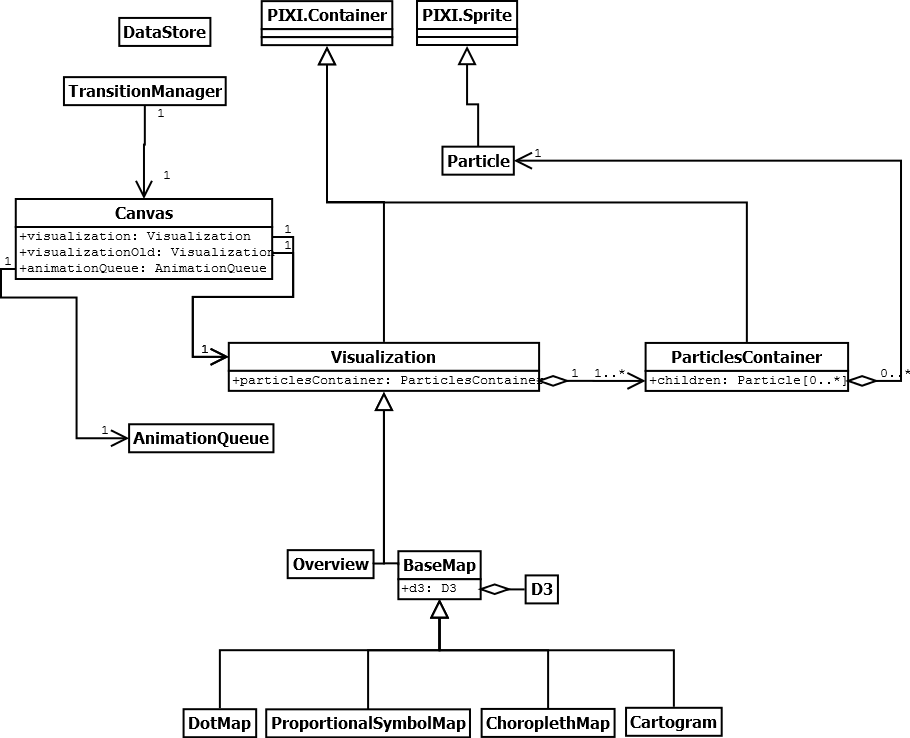
\includegraphics[width=0.8\textwidth,keepaspectratio]{images/results/dia.png}
\caption[
    Overview of the application architecture in the form of a class diagram.
]{Overview of the application architecture in the form of a class diagram.}
\label{fig:uml-practical-approach}
\end{figure}
%TC:endignore

\begin{description}
\item[DataStore] \hfill \\
An object of the DataStore-class is used to load the SuperStore-Sale dataset. In addition to initally loading it, it also parses and analyses the dataset. Each attribute of the dataset got classified to handle the attributes correctly later on. For the sake of convenience, three different classification types were used: numeric, date, nominal and unknown.

\item[PIXI.Container] \hfill \\
\ac{Pixi} features functionalities like container classes. \textit{PIXI.Container} is such a class and can be used to put objects in it, and scale or move those objects according to the base-canvas.

\item[AnimationQueue] \hfill \\
If an animation is assigned to particles, it is stored in the \textit{AnimationQueue}. This allows to create multiple canvas-based animations and process them sequential.

\item[Canvas] \hfill \\
This class is one of the main classes inside the application. It is needed to not compare it with an HTML-Canvas object. However, this class is responsible for creating the base-canvas of the web-application. Furthermore, it is used to change and update the visual appearance if any interaction happens. A key part of the canvas class is the render function shown in listing \ref{lst:canvas-render} on page \pageref{lst:canvas-render}. It starts off with calling the same function again as soon as possible. The caller-function \textit{requestAnimationFrame} ensures, that the next frame will only be shown if enough resources of the browser are available. Afterwards, all particles and visualisations are animated if something changed. The last line of the listing shows the \ac{Pixi}-renderer. Listing \ref{lst:canvas-autodecet-renderer} on page \pageref{lst:canvas-autodecet-renderer} shows its creation. It features the main canvas-size, background transparency, antialiasing and a lot of other options.

%TC:ignore
\begin{lstlisting}[language=JavaScript, caption={Render function of the canvas class.}, label={lst:canvas-render}]
    render() {
      this.requestFrameID = requestAnimationFrame(this.render.bind(this));

      let areParticlesAnimating = this.particlesContainer.nextStep();
      let isNewVisualizationAnimating = this.visualization.nextStep();
      let isOldVisualizationAnimating =  ? this.visualizationOld.nextStep() : false;

      if (!areParticlesAnimating && !isOldVisualizationAnimating &&
        !isNewVisualizationAnimating && this.animationQueue.length > 0) {

        this.animationQueue.pop()();
        this.particlesContainer.startAnimation();
        this.visualization.startAnimation();
        if (this.visualizationOld){
            this.visualizationOld.startAnimation();
        }
      }
      this.renderer.render(this.stage);
    }
\end{lstlisting}

\begin{lstlisting}[language=JavaScript, caption={Pixi's autodetect-renderer.}, label={lst:canvas-autodecet-renderer}]
    this.renderer = PIXI.autoDetectRenderer(this.width, this.height, {
        transparent: true,
        clearBeforeRender: true,
        antialias: true
    });
    document.body.appendChild(this.renderer.view);
\end{lstlisting}
%TC:endignore

\item[Visualization] \hfill \\
This class is the starting point and the parent class for all other types of visualisations. It stores a reference to the \textit{ParticleContainer} and provides functionality to move, scale or change visualisations.

\item[Overview] \hfill \\
Creating an instance of \textit{Overview} will show all data items as unit-based grid.

\item[D3] \hfill \\
This class is mainly used to wrap all functionality of the \ac{D3} library. It features functions like initialising the base-map as a \ac{SVG} and loading the needed TopoJSON data accordingly. \ac{D3} offers multiple projections for GeoJSON data. Listing \ref{lst:d3-map-init} on page \pageref{lst:d3-map-init} shows a part of the map initialisation with the projection used. The projection is an extension of an Albers equal-area projection discussed in chapter \ref{s:map-projections} on page \pageref{s:albers-equal-area-projection}. It is a United-States-centric composite projection. The lower forty-eight states of america are projected using the default Albers-equal-area projection. However, Alaska and Hawaii use a separate conic equal-area projection. The scale of Alaska is furthermore diminished. It is projected at $0.35\times$ its true relative area. The scale and translation of the map are set to use the available window space and center the map on the screen.

%TC:ignore
\begin{lstlisting}[language=JavaScript, caption={Map initialisation with a map projection, scale, and translation.}, label={lst:d3-map-init}]
    this.projection = this._d3.geo.albersUsa()
        .scale(width)
        .translate([this.width / 2, this.height / 2]);
\end{lstlisting}
%TC:endignore

Another key part of this class is featured in listing \ref{lst:d3-topojson} on page \pageref{lst:d3-topojson}. It shows how TopoJSON is used on the client. The filter function passed to the first \textit{TopoJSON.mesh}-function specifies that only internal state borders should be drawn. Thus, coastlines will not be drawn to retain detail around small islands and inlets. The filter function passed to the second \textit{TopoJSON.mesh}-function extends the first one by only drawing each county boundary once. Thus, if two counties share the same border, it is only drawn once.

%TC:ignore
\begin{lstlisting}[language=JavaScript, caption={TopoJSON usage on the client with the adaption of merging all geographic information.}, label={lst:d3-topojson}]
    this.data.topojson.states = topojson.mesh(
        this.data.us,
        this.data.us.objects.states,
        (a, b) => {
            return a !== b;
        }
    );

    this.data.topojson.counties = topojson.mesh(
        this.data.us,
        this.data.us.objects.counties,
        (a, b) => {
            return (
                a !== b &&
                !(this.getCountyIdentifier(a) / 1000 ^ this.getCountyIdentifier(b) / 1000)
            );
        }
    );
\end{lstlisting}
%TC:endignore

Another important aspect of the \ac{D3} class is the \textit{calculateCentroids}-function shown in listing \ref{lst:d3-calculate-centroids} on page \pageref{lst:d3-calculate-centroids}. It calculates a look-up dictionary for the given level of detail for each data item. Thus, providing a huge performance boost when finding out the centroid of a unit later on.

%TC:ignore
\begin{lstlisting}[language=JavaScript, caption={Calculate a look-up dictionary for all data items depending on the level of detail.}, label={lst:d3-calculate-centroids}]
    calculateCentroids(levelOfDetail){
        const boundaries = this._topojson.feature(
            this.data.us,
            this.data.us.objects[levelOfDetail]
        ).features;

        this.centroids[levelOfDetail] = {};
        for(let boundary of boundaries){
            this.centroids[levelOfDetail][boundary.id] = this.path.centroid(boundary);
        }
    }
\end{lstlisting}
%TC:endignore

% SYMBOL SCALE AND COLOR SCALE TO SHOW

\item[BaseMap] \hfill \\
This is the second class inheriting from the \textit{Visualization} class. It features a single object of the \ac{D3} class. Therefore, it is possible that all deriving classes share the same object of \ac{D3} and thus, all its features and settings. Changing the level of detail of the \textit{BaseMap} will affect the map initialised in \textit{\ac{D3}} and hence, all deriving classes are using the same base-map again. This class is mainly used to share the same object of \ac{D3} for all children.
The decision if the upcoming map should be animated or not handles each subclass on its own. All of them use the same concept of determining the type of transition: each implemented subclass has some kind of \textit{draw}-function which accepts an optional parameter called \textit{animationCb}. If this parameter exists and is not \textit{undefined}, the transition to the upcoming visualisation is animated.
All subclasses based on aggregation are implemented and animated with \ac{D3}. Therefore, dot map is slightly different than these in the terms of structure and usage. Furthermore, all thematic maps based on aggregation are implemented with the method of using a static file consisting of all information. However, the aggregated values could also be calculated every time.

\item[DotMap] \hfill \\
The \textit{DotMap} class is the first one to show data on the base-map. It does not use the \ac{DOM} to create the units on the map. It uses the already existing particles from the particle container inherited from the \textit{Visualization} class. Key part of this class is the determination of animating particles or not.
The herein before mentioned decision if particle should be animated or not is shown in listing \ref{lst:dot-draw-animated} on page \pageref{lst:dot-draw-animated}. It also shows the further executed actions if they should be animated, like projecting the longitude and latitude of the point onto the map and calling the main \textit{draw}-function for each particle.

%TC:ignore
\begin{lstlisting}[language=JavaScript, caption={Particles on a dot map getting animated.}, label={lst:dot-draw-animated}]
    if(this.isFunction(animationCb)){
        for(let particle of this.particles){
            point = [particle.data.Longitude, particle.data.Latitude];
            point = this.baseMap.projection(point);
            particle.coords = point;

            setTimeout(drawFunc.bind(this), 250, particle, this.size);
        }
    }
\end{lstlisting}
%TC:endignore

\item[ProportionalSymbolMap] \hfill \\
Drawing proportional symbols is done by using \ac{D3}. First of all, it does not use the SuperStore-Sale file as a basis, and instead uses the preprocessed TopoJSON file. The \textit{draw}-function of this class gets two parameters: the level of detail which should be drawn and the decision if the symbols should be animated. Listing \ref{lst:psm-draw} on page \pageref{lst:psm-draw} shows how each circle for the proportional symbol map is drawn and eventually animated. Line 8-13 loads the already existing data into the created \ac{SVG}-element. It is important to sort the data first because if this would not happen, bigger circles would cover smaller ones. Drawing the bigger ones first results in zero overpainting. The \textit{.data()}-function returns an array. Iterating through every item in the array is done with the \textit{.enter()}-method. Line 15 and onwards create a proportional symbol called \textit{circle} for each data item in the array. They set its position with \textit{transform} and decide, if its radius should be animated or not.

%TC:ignore
\begin{lstlisting}[language=JavaScript, caption={The draw-function of the ProportionalSymbolMap-class}, label={lst:psm-draw}]
    draw(id, animationCb){
        let map = this.baseMap;

        this[id] = map.svg.append("g")
        .attr("id", `psm-${id}`)
        .attr("class", "bubble")
        .selectAll("circle")
        .data(
            map._topojson.feature(map.data.us, map.data.us.objects[id]).features
            .sort(function(a, b) {
                return (b.properties.orders || 0) - (a.properties.orders || 0);
            })
        )
        .enter()
        .append("circle")
        .attr("transform", function(d) {
            let coords = map.path.centroid(d);
            if(isNaN(coords[0]) || isNaN(coords[1])) return;
            return "translate(" + coords + ")";
        });

        if(this.isFunction(animationCb)){
            this[id]
            .attr("r", 0)
            .transition()
            .delay(300)
            .attr("r", function(d) {
                return map.symbolScale(d.properties.orders) || 0;
            })
            .each("end", animationCb);
        } else {
            this[id]
            .attr("r", function(d) {
                return map.symbolScale(d.properties.orders) || 0;
            });
        }
    }
\end{lstlisting}
%TC:endignore

\item[ChoroplethMap] \hfill \\
The implementation of this type of thematic map is a classified choropleth map. As all the other versions of aggregated thematic maps, the distinction between animated and static drawing is done. Listing \ref{lst:choropleth-part-draw} on page \pageref{lst:choropleth-part-draw} shows a small part of the \textit{draw}-function. If the \texit{animationCb} is truthy, all enumeration units are first coloured with a light grey, followed by a colour transition based on the orders of the unit.

%TC:ignore
\begin{lstlisting}[language=JavaScript, caption={The draw-function of the ProportionalSymbolMap-class}, label={lst:choropleth-part-draw}]
    if(this.isFunction(animationCb)){
        this[id]
        .attr("fill", "#D3D3D3")
        .transition()
        .delay(300)
        .duration(1000)
        .attr("fill", d => {
            let scaled = map.colorScale(
                map.symbolScale(Number(d.properties.orders) || 0) || 0
            );
            return this.getColor[scaled];
        })
        .each("end", animationCb);
    } else {
        this[id]
        .attr("fill", d => {
            let scaled = map.colorScale(
                map.symbolScale(Number(d.properties.orders) || 0) || 0
            );
            return this.getColor[scaled];
        });
    }
\end{lstlisting}
%TC:endignore


\item[Cartogram] \hfill \\
The web-application implements a specific type of cartogram: a pseudo Demers cartogram. A true Demers cartogram would need links between adjacent features. However, the type of cartogram implemented tries to preserve locality instead of connectedness. Therefore, each square is located as close as possible to its origin without overlapping. In order to deliver this kind of information to the user, a collision detection with gravity is used to animate the position of each square. Listing \ref{lst:cartogram-part-draw} on page \pageref{lst:cartogram-part-draw} shows a small part of the \textit{draw}-function. It covers the part of initially drawing each square and afterwards starting the collision detection and the gravity.

%TC:ignore
\begin{lstlisting}[language=JavaScript, caption={The draw-function of the pseudo Demers Cartogramm-class}, label={lst:cartogram-part-draw}]
    this.node = map.svg.append("g")
    .attr("id", `cartogram-${id}`)
    .selectAll("rect")
    .data(this.nodes)
    .enter()
    .append("rect")
    .attr("class", "rect");

    if(this.isFunction(animationCb)){
        this.node
        .attr('width', 0)
        .attr('height', 0)
        .transition()
        .delay(300)
        .attr("x", d => { return d.x - d.r; })
        .attr("y", d => { return d.y - d.r; })
        .attr("width", d => { return d.r * 2; })
        .attr("height", d => { return d.r * 2; })
        .each("end", () => {
            animationCb();

            force
            .nodes(this.nodes)
            .on("tick", this.tick.bind(this, 0.00599))
            .start();

        });
        this[id] = this.node;
    }
\end{lstlisting}
%TC:endignore

\item[ParticlesContainer] \hfill \\
This container contains all particles and ensures, that they are animated in the desired order. Furthermore, it controls the speed of each animated particle.

\item[Particle] \hfill \\
A particle is inherits the functionality of \textit{PIXI.Graphics} and contains information about its position, alpha value, and the data it represents. It exposes methods to draw a particle onto the map and to animate it.

\end{description}

% As one can see, all thematic maps based on aggregation keep a reference of the data shown. Therefore, changing the level of detail first checks, if the map needs to be updated or not.

\subsubsection{Interaction}
% transition
% level of detail
% changing visual appearance

\subsection{User study}
To answer the research question of this thesis, a user study yielding qualitative results was conducted. Such a study verifies that the implemented application fulfills its design goals.
The study setup was held in a laboratory environment with 14 participants. It was necessary that each participant does not know the purpose of proportional symbol maps, choropleth maps and cartograms. This requirement ensures that recognition of the animated transition between two visualisations is not combined with previous knowledge about the thematic map type.

The design of the conducted study was within-subject with think-aloud tasks and a post-task interview. Its primary objective was to check if participants understand the relationship between different geo-spatial visualisations and also help them to extract strengths and weaknesses of each visualisation type. To achieve this, the task participants had to solve was of minor importance. It consisted of finding one of the areas in the United States with the most orders normalised by population. Participants had to justify their answer with the chosen map type. Although, each implemented type of map would be sufficient to answer the question, another requirement was introduced. Participants had to look at every map type at least once. The justification of their answer lead to a post-task interview, where they were asked why they did or did not choose a specific type of map. The participants had to name the advantages and disadvantages of each thematic map if possible (as shown in Chapter \ref{s:univariate-maps} on page \pageref{s:univariate-maps}).
To conclude the study, they had to rate the usefulness of the transitions on a scale from 1 to 5 where 1 denotes the transition as unhelpful and 5 as helpful. Hence, the results of the user study are in a binary format - either a participant could name a particular advantage or disadvantage or not and include a score for the transition overall.

The conducted user study was performed with six female and eight male participants. They were between 21 and 47 years old. They all described themselves as technically affine with some experience in the domain of information visualisation and no experience with transitions between visualisations. The residual chapter shows the results from the study.

Revealing a general pattern of a distribution is the main objective of a dot map. 10 out of 14 participants could name the purpose of this thematic map. Even more participants (11 out of 14) said that it is not possible to determine exact quantities in a dot map due to underestimation of high density areas.

The major drawback of a proportional symbol map was detected by 10 out of 14 attendees. According to their feedback, the east coast of the United States was very hard to read due to close locations with high population and therefore overlapping symbols. However, only six people found that the estimation of quantities is less tedious. Seven people were able to name the advantage of a non-existing areal bias.

Finding hot spots was identified by 100\% of the participants as the primary goal of a choropleth map. Furthermore, nine attendees could also name the areal bias as a disadvantage of a choropleth map.

The distortions a cartogram comes along with are identified by 12 attendees as the main weakness of this type of map. Nonetheless, three participants discovered that cartograms emphasise the attribute mapped to the size of the symbol and eliminate visual biases due to their abstractness.

In addition, 10 participants rated the transition between the thematic maps with a score between three and five. The mean score of the transition is 3,21.

